\chapter{Implementation}
\label{sec:implementation-chapter}

This chapter is dedicated to introducing the implementation
of the proposed branch-and-cut algorithm.
As the main foundation, the proposed approach employs
the latest \textit{CPLEX 22.1 C callable library} (released in March 2022).
The branch-and-cut framework can be used as a pricer in the context
of column generation for the CVRP.
The algorithm's source coed is developed in the \textit{C} language,
and it is freely available under a permissive \textit{MIT} license
at the following Github repository: \url{https://github.com/dparo/master-thesis}.

\begin{quote}
	The BAC algorithm is implemented using callback functions for cut gen-
	eration which is available in the CPLEX callable library \cite{jepsen2008branchandcut}.
\end{quote}

\medskip

\urlref{https://www.ibm.com/analytics/cplex-optimizer}{IBM ILOG CPLEX Optimizer},
CPLEX for short,
is a commercial optimization software package for solving problems expressed as either:
linear programs, mixed-integer programs, quadratic programs, or quadratic constrained programs.
For an introduction to CPLEX refer to \Cref{sec:introduction-to-cplex}.
Compared to tailored pricers, such as the labeling algorithm \parencite{desrochers1992, feillet2004},
it is clear that using a modern MIP solver, such as CPLEX,
may provide at least two benefits:
(i) parallelization and efficient use of the machine' multiple cores basically for free,
(ii) take advantage of all the engineering effort that went in creating an efficient MIP solver.

\medskip

We quickly summarize the outline of the chapter.
\Cref{sec:impl-full-static-model} presents the implemented static IP model,
which is based on the CPTP formulation previously described in \cref{sec:the-capacitated-profitable-tour-problem}.
\Cref{sec:impl-warm-starting} describes the primal heuristics employed
to warm start the CPLEX optimizer.
\Cref{sec:impl-branching} describes the employed branching schemes.
Finally, \cref{sec:impl-separation-techniques} describes the cutting-planes,
including their separation,
aimed at improving the linear relaxation.

\section{Full static model}
\label{sec:impl-full-static-model}

Our branch-and-cut based pricer makes of a static IP model
based on the CPTP formulation of \labelcref{eq:cptp-obj-function,eq:cptp-depot-part-of-tour-constraint,eq:cptp-resource-upper-bound-constraint,eq:cptp-flow-conservation-constraint,eq:cptp-gsec-constraints,eq:cptp-x-mip-var-bounds,eq:cptp-y-mip-var-bounds}
disregarding the GSECs of \cref{eq:cptp-gsec-constraints};
see discussion in \cref{sec:the-capacitated-profitable-tour-problem} for more details.
To guarantee the correctness of the approach,
the GSECs will be dynamically separated on violation
during the running-time of the branch-and-cut algorithm.
Note that to guarantee the correctness of the approach,
the GSECs must be separated through an exact procedure
(at least for the integral solutions).
We've implemented the following static Integer Programme (IP) model:
\begin{align}
	\min_{x,y} \quad z_\mt{CPTP}(x, y) & = \ExprCptpObjValDef                     & \label{eq:cptp-static-model-0}                         \\
	                                   & y_0 = 1                                  & \label{eq:cptp-static-model-1}                         \\
	                                   & B \le   \ExprCptpDemandSum   \le Q       & \label{eq:cptp-static-model-2}                         \\
	                                   & \ExprCptpEdgesIncident{i}    = 2 y_i     & \quad \forall i \in V  \label{eq:cptp-static-model-3}  \\
	                                   & x_{e}                   \in \Set*{0, 1}  & \quad \forall e \in E  \label{eq:cptp-static-model-4}  \\
	                                   & y_{i}                    \in \Set*{0, 1} & \quad \forall i \in V  \label{eq:cptp-static-model-5},
\end{align}
where
$B \in R_+$ is an additional lower bound on the resource consumption
that may help in gaining a slight improvement on the linear relaxation.
The value of $B$ is computed as $B = q_u + q_v$, where $u, v \in V_0,\ u \ne v$
represent the least two demanding customers in the network:
$q_u \le q_v \le q_i \quad \forall i \in V_0, i \ne u, v$.

\subsection{Upper cutoff value}
\label{sec:impl-upper-cutoff-value}

In the context of pricing for the CVRP,
we're only interested in routes achieving a strictly negative cost function.
The upper cutoff value can help a MIP optimizer
in reducing the number of evaluated branch-and-bound nodes.
The upper cutoff value behaves as a constraint specified directly on the objective function:
\begin{equation}
	z_\mt{CPTP}(x, y) \le 0 - \varepsilon_{\mt{ct}},
\end{equation}
where $\varepsilon_{\mt{ct}} \in \R_+$ is the upper cutoff tolerance.
Most MIP solvers, including CPLEX, has internal support for specifying cutoff values.
However, it is important to note that specifying the cutoff value is not identical
to specifying an explicit constraint in the static model.
Cutoff values contribute only when the branch-and-bound procedure is invoked.
Whereas, an explicit constraint contributes even at the linear relaxation level.
The upper cutoff tolerance $\varepsilon_{\mt{ct}}$ biases the threshold at which the produced
route can be considered a valid reduced cost column.
A non-zero value for $\varepsilon_{\mt{ct}}$ avoids numerical
stability problems caused by the usage of floating point arithmetic
employed in BPC implementations.
To guarantee correctness, the value of $\varepsilon_{\mt{ct}}$ should match the
value employed by the BPC algorithm.
In our case we picked $\varepsilon_{\mt{ct}} = 10^{-6}$,
since it is the value used by the modern BPC framework presented in \textcite{sadykov2021}.

\section{Warm Starting}
\label{sec:impl-warm-starting}

\textit{Warm starting} is a process which consists in feeding
a MIP optimizer with (good) feasible solutions
prior to starting the resolution process.
Having a set of (good) initial feasible solutions,
can help a modern MIP solver to reach optimality in less time,
Warm starting, if properly implemented,
can tremendously reduce the primal-dual bound gap for many problem domains.

Primal heuristic algorithms provide a fast and sensible approach for warm starting.
A CPTP problem has many similarities with TSP.
Therefore,
TSP's heuristics can be readjusted to work successfully even for the CPTP.
Much work was dedicated in studying good heuristics for the TSP,
see \cite{rosenkrantz1977, johnson1997, laporte1992, johnson2007, hoffman2013}.

In the remainder of this section,
we explain the warm starting procedure that we've implemented.
The procedure is characterized by two stages:
a constructive insertion heuristic stage (see \cref{sec:impl-insertion-heuristic})
followed by a 2-OPT refinement stage (see \cref{sec:impl-2opt-refinement}),

\subsection{Insertion heuristic}
\label{sec:impl-insertion-heuristic}

\cite{rosenkrantz1977} do a fantastic job in describing the insertion heuristic algorithm
for the TSP and various facets in which it can be implemented.
The insertion heuristic algorithm
can construct a new feasible primal solution in $\Theta(N^2)$ time.
In this section,
we will focus on readjusting the TSP insertion heuristic so that it can work with a CPTP problem.

\medskip

Start by selecting two distinct nodes $u, v \in V,\ q_u + q_v \le Q$
to form an initial tour back-to-back $p = \Tuple*{u, v}$.

The insertion heuristic is an iterative approach,
where at each step of the iteration
an almost-feasible CPTP tour is available.
If the CPTP admits feasible solutions,
when all the iterations of the insertion heuristic are exhausted,
the final available tour will surely be CPTP feasible.
Let's define $q(p) \le Q$ as the total demand served
in by the partial route in the current iteration.
At each iteration,
choose a vertex $a \in p$ and a vertex $h \notin p$.
Let's define $b$ as the successor of node $a$ in the current tour.
The idea is to try to insert $h$ in the tour,
by deleting edge $\Tuple*{a, b}$
and inserting edges $\Tuple*{a, h},\ \Tuple*{h, b}$.
The insertion operation should be performed only
if the $h$ insertion is mandatory to restore feasibility,
or alternatively if it's insertion lowers the route cost.
More formally, let's define the extra mileage as:
\begin{equation}
	\Delta_m(h, a) =
	\begin{cases}
		c_{ah} + c_{hb} - c_{ab} - p_h, & \texttt{if } q(p) + q_h \le Q \\
		\infty,                         & \texttt{otherwise},
	\end{cases}
\end{equation}
which represents the delta route cost in inserting $h$ as the successor of node $a$.
A vertex $h \in V$ is a good candidate for insertion
if at least one of the following conditions is true:
\begin{enumerate}
	\item $\Delta_m(h, a) < 0$, i.e. inserting $h$ improves over the current route.
	\item $h = 0$, i.e. $h$ is the depot node.
	      The depot node at some point must be inserted regardless whether it is improving or not.
	      Note that by convention we have defined $q_0 = 0$,
	      therefore $q(p) + q_0 \le Q$ is always satisfied for the depot node.
	\item The number of visited nodes in the current tour is $2$ and $q(p) + q_h \le Q$.
\end{enumerate}

Prior to insertion the partial route has the form $p = \Tuple*{\dots, a, b, \dots}$;
whereas after the insertion operation completes: $p = \Tuple*{\dots, a, h, b, \dots}$.
In our implementation we employed the cheapest insertion scheme,
therefore the pair $(h, a)$ for is picked such that it minimizes the extra mileage $\Delta_m(h, a)$
across all possible choices for $a \in p,\ h \notin p$.
The iteration stops when no more valid $h$ vertices can be found for insertion.
At the end of the insertion heuristic, $p$ is a valid route which visits the depot node.
Note that the depot node may not necessarily be the first element of the tour: $p_0 \ne 0$.
A simple circular rotation is sufficient to restore the condition $p_0 = 0$.
It may happen that no valid $h$ can be found,
yet the current tour length is $2$.
In this very unlikely scenario,
we can conclude that the CPTP formulation does not admit any feasible solution
before even solving the IP formulation.

In our implementation we picked $u = 0$ and $v \in V_0$, such that $q_u + q_v \le Q$.
This allows us to generate $O(N)$ good feasible primal solutions using insertion heuristic in $O(N^3)$ time.

\subsection{2-OPT refinement}
\label{sec:impl-2opt-refinement}

Each solution produced from the insertion heuristic
can be further improved using a \textit{2-OPT refinement procedure}.
The 2-OPT algorithm is a heuristic local-search hill-climbing procedure
proposed originally for the TSP in \textcite{flood1956, croes1958} independently.

The 2-OPT algorithm works iteratively requiring $\Omega(N^2)$ number of iterations.
Unfortunately,
as it is pointed out in \textcite{chandra1999},
the 2-OPT procedure may in the worst case take an exponential number of iterations
when fed with purposely artificially constructed instances.
Although this is bad news,
it is also worth pointing out that this rarely occur in practice,
as the probabilistic average number of iterations required for 2-OPT is at most polynomial.

Each iteration of the 2-OPT procedure searches for an existing edge crossing,
and if any exists,
it performs a 2-OPT exchange to undo it.
A 2-OPT exchange is a \textit{primal operation},
i.e. its application preserves route feasibility.
A 2-OPT exchange does not add nor remove vertices from the current route $p$,
therefore the route's gained profit does not change during
the running time of the 2-OPT procedure.
Hence, it is trivial to readjust the original TSP's 2-OPT procedure to the CPTP problem.

Let $a, b \in p$ be two vertices visited in the current route.
Let $a^\prime, b^\prime \in p$ denote respectively the successor of $a$ and $b$ in the current route.
A 2-OPT exchange removes edges $(a, a^\prime)$, $(b, b^\prime)$
in favor of $(a, b)$, $(a^\prime, b^\prime)$
but only if the delta distance, defined as:
\begin{equation}
	\Delta(a, b) = c_{a b} + c_{a^\prime b^\prime} - c_{a a^\prime} - c_{b b^\prime},
\end{equation}
satisfies $\Delta(a, b) < 0$.
If this is the case, performing a 2-OPT exchange over vertices $(a, b)$ lowers the route cost.
After a 2-OPT exchange,
it is necessary to reverse the portion of the route
characterized from the head $a_s$ and tail $b$: $[a_s, \dots, b]$.

In our implementation
we scan for vertices $a, b$ achieving the cheapest exchange,
i.e. for which the delta distance $\Delta(a, b)$ is minimized across all possible valid choices of $a, b \in p$.

\section{Branching}
\label{sec:impl-branching}

We don't implement any specific branching schemes.
We rely on the branching schemes already provided from the CPLEX MIP optimizer.

\mytodo{Strong branching employed?}

\section{Cutting-planes separation}
\label{sec:impl-separation-techniques}

Despite separation of some general families of cutting-planes are already provided
from modern MIP optimizers such as CPLEX, such as:
Chvátal-Gomory cuts, mixed integer rounding cuts, disjunctive cuts
and cover inequalities (see \cref{sec:introduction-to-cplex});
reporting additional inequalities, which cannot be deduced from the static model,
can drastically improve the running time of the resolution process.


The GSECs can be separated for fractional solutions by solving $(s, t)$-min-cuts
on a flow network where capacities are given from the fractional solution $x^\star$.

No exact separation procedure is currently known RCC inequalities \parencite{jepsen2014}.

GLM separation is sub-optimal because  the capacities
of the flow network need to also account for the demand of the vertices.

Despite the are no exact separation procedure known for the RCC inequalities,
we take the approach taken in \textcite{jepsen2014},
and use min-cuts to separate this family of inequalities.
Despite this procedure may be suboptimal, it has the specific
benefit that the same labeling procedure employed in the GLM separation,
can also be used for this family of cuts.

\begin{comment}
\cite{jepsen2014}
The BAC algorithm is implemented within CPLEX 12 using the callback functions for the cut generation
from the callable library.
\end{comment}

\begin{comment}
\cite{ralphs2003}
The most important and challenging aspect of any branch and cut algorithm is designing
subroutines that effectively separate a given fractional point from the convex hull of
integer solutions. This has been, and still remains, a very challenging aspect of applying
branch and cut techniques to the VRP.
\end{comment}

Inequality separation is a problem which consists in finding (strong) violated inequalities so that they can be embedded inside a Branch\&Cut framework.
Integral inequality separation is concerned in determining violated inequalities for the original IP model.
Integral inequalities' separation is usually much easier to perform, and can be seen as a procedure to dynamically generate necessary constraints that would otherwise be impossible to insert statically in a MIP model.
Fractional inequality separation, instead is usually harder to perform, and it is concerned in finding (strong) violated inequalities for fractional solutions originated from the linear relaxation.

In this thesis we are treating a CPTP problem, and more precisely, we are concerned in separating the GSEC, GLM, RCC inequalities presented in Sections \ref{sec:gsec-inequality}, \ref{sec:additional-valid-inequalities}.
This is achieved by finding sets $S \subseteq V_0$, through the usage of appropriate algorithms, that violate any valid inequality.

All the cuts that we implemented, are backed by the same shared separation procedure for both integral solutions and for fractional solutions.
In the next two sections, we describe the common separation procedure used to find good $S \subseteq V_0$ sets.
Then for each cut, we describe: how $S$ is used for generating the inequality and when each cut is reported to the MIP solver or when it is, instead, ignored.

\subsection{Integral separation}
\label{sec:impl-integral-separation}

The integral separation procedure is the most important, as this procedure is necessary to generate GSEC inequalities dynamically, which have the effect of rejecting solutions containing spurious unconnected subtours.
Assume that the MIP solver finds an optimal integer solution $x^* \in \Set*{0, 1}, y^* \in \Set*{0, 1}$ that violates a GSEC constraint.
If $x^*$ violates at least a GSEC, it is easy to see that the solution models at least a spurious unconnected subtour that needs to be removed.
In order to detect unconnected subtours, we need first to determine the connected components induced from the $x^*$ solution.

Let $C = \Set*{-1, 0, \dots, n_c - 1}$ be the connected components formed with $n_c \ge 1$.
A node $i$ is said to belong to a singleton connected components, if the connected component contains only $i$ itself.
We are only interested in modeling \textbf{major} connected components, i.e. components containing at least two vertices.
Therefore, we ignore singleton connected components, and we use the sentinel value $-1$ for all the nodes $i$ belonging to singletons.
Thus, the $n_c$ represents the number of major connected components, i.e. the number of subtours formed in the current integral solution.
Let $cc(i) \in C$ be an array which for each vertex $i \in V$ it encodes to which connected component it belongs to.
Note that the depot node always belongs to a connected component, therefore by definition we fix $cc(0) = 0$.
For singletons instead we fix $c(i) = -1  \quad \forall i \in V_0 \mid y_i = 0$.
The connected components can be computed by a simple depth first search traversal, for which a pseudocode is provided in Algorithm \ref{algo:cc-dfs}.

\begin{algorithm}
	\caption{An algorithm for computing the connected components through a DFS traversal}
	\KwData{$x^*, y^* \in \{0, 1\}$: current integral solution of
		\cref{eq:cptp-static-model-0,eq:cptp-static-model-1,eq:cptp-static-model-2,eq:cptp-static-model-3,eq:cptp-static-model-4,eq:cptp-static-model-5}
	}
	\KwResult{$n_c$: number of subtours formed}
	\KwResult{$cc[i] \in C$: connected component of $\forall i \in V$}
	\Proc{\textit{cc\_dfs}($x^*$, $y^*$)}{
	\Let $cc[i] \gets -1 \quad \forall i \in V$\;
	\Let $nc \gets 0$\;
	\For{$i\gets0$ \KwTo $N$}{
		\If{$cc[i] < 0, y^*_i = 1$}{
			\Comment{Found a non visited sub-tour}
			$cc[i] \gets n_c$\;
			\Let $u \gets -1$\;
			\Comment{Traverse the sub-tour}
			\Do{$u \ge 0$}{
				\Let $v \gets -1$\;
				\For{$j \in V \mid e = \Set*{u, j} \in E,\ cc[j] < 0,\ x^*_{e} = 1$}{
					\Comment{The body of this loop will execute only once}
					$cc[j] = n_c$\;
					$v \gets j$\;
				}
				$u \gets v$
			}
			$n_c \gets n_c + 1$\;
		}
	}

	\Comment{Validate some invariants}
	\Assert{$n_c \ge 0$}\;
	\Assert{$c[0] = 0$}\;
	\Assert{$c[i] = -1 \quad \forall i \in V_0 \mid y^*_i = 0$}\;
	\Assert{$c[i] \ge 0 \quad \forall i \in V_0 \mid y^*_i = 1$}\;
	\Comment{Done: terminate}
	\Return{$n_c, cc$}
}

	\label{algo:cc-dfs}
\end{algorithm}

Then any valid set $S \in V_0$ can be computed in the following way from a MIP integer solution:

\begin{equation}
	S \subseteq V_0 = \Set* {i \mid cc(i) = k}   \quad \forall k \in C, k > 0
\end{equation}

which implies that any major connected component that does not contain the depot node, can be used as a valid set $S \subseteq V_0$ for separating inequalities.
If $n_c = 1$ then no $S \subseteq V_0$ can be separated for this integral solution, which in our case simply means that the solution contains a single subtour, and does not violate any GSECs.
A block diagram summarizing the integral separation is provided in \cref{fig:integral-separation-block-diagram}.

\begin{figure}[ht]
	\centering
	\framebox{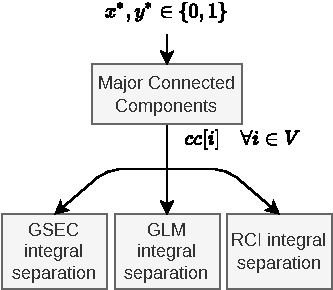
\includegraphics[width=6cm]{Imgs/integral-separation-block-diagram.cropped.pdf}}
	\caption{A block diagram representing the structure of the employed integral separation procedure.}
	\label{fig:integral-separation-block-diagram}
\end{figure}

\subsection{Fractional separation}
\label{sec:impl-fractional-separation}

Fractional separation is usually much harder and more computationally expensive to perform compared to integral separation.
A valid set $S \subseteq V_0$ can be separated by solving a max-flow problem between two arbitrary source and sink vertices $s, t \in V,\ s \ne t$ on a fully connected directed graph.
Fractional separation is modeled through a directed symmetric flow network, where $x^*_{ij}$, i.e. the current fractional solution, constitutes the capacities of the flow network.

A solution to the max-flow problem outputs a maxflow $\maxflow(s, t)$ and a bipartition, also called "coloring", of the set $V$, namely two complementary sets $F_1(s, t), F_2(s, t)$ such that $F_1(s, t) \cup F_2(s, t) = V$ and $F_1 \cap F_2 = \emptyset$, and such that $s \in F_1(s, t),\ t \in F_2(s, t)$.
The $\delta(F_1(s, t))$ constitutes the min-cut induced from solving the max-flow problem over $(s, t)$.
It is known that solving a maxflow problem guarantees the following two properties:

\begin{enumerate}
	\item Edges $\{ (i, j) \mid i \in F_1(s, t),\ j \in F_2(s, t) \}$ are saturated
	\item Edges $\{ (j, i) \mid i \in F_1(s, t),\ j \in F_2(s, t) \}$ are drained.
\end{enumerate}

therefore the following result holds:
\begin{align}
	\sum_{(i, j) \in \delta(F_1(s, t))} f_{ij} & = \maxflow(s, t) \\
	\sum_{(i, j) \in \delta(F_2(s, t))} f_{ij} & = 0
\end{align}

where $f_{ij}$ denotes the flow along the edge $(i, j),\ i, j \in V$ in the corresponding flow network.
Assuming we have already computed $F_1(s, t), F_2(s, t)$, a valid $S \subseteq V_0$ can then be picked such that:
\begin{equation}
	S \subseteq V_0 =
	\begin{cases}
		F_1(s, t), & \texttt{if } 0 \notin F_1(s, t) \\
		F_2(s, t), & \texttt{otherwise}
	\end{cases}
\end{equation}

This fractional separation framework based on max-flow computations, can separate up to $N^2 - N$ different $S \subseteq V_0$ sets, one for each possible choice of $s, t \in V, s \ne t$.
It is important to note that, since we are dealing with a \textbf{symmetrical} flow network, solving the maxflow problem between pairs $(s, t)$ and pair $(t, s)$ will output the same maxflow, i.e. $\maxflow(s, t) = \maxflow(t, s)$.
Although, and this is the more important aspect, the induced bipartitions in the general case are not guaranteed to be symmetric.
Namely, in general, $F_1(s, t) \ne F_2(t, s)$ and $F_2(s, t) \ne F_1(t, s)$.
To see this is the case, this simple flow network:

\begin{center}
	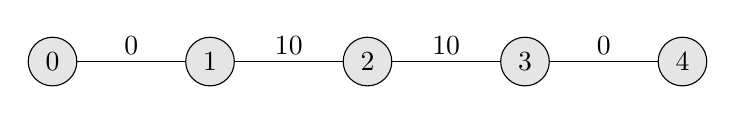
\begin{tikzpicture}[node distance={20mm}, main/.style = {draw, circle, fill=black!10!white}]
		\centering

		\node[main] (0) {$0$};
		\node[main] (1) [right of = 0] {$1$};
		\node[main] (2) [right of = 1] {$2$};
		\node[main] (3) [right of = 2] {$3$};
		\node[main] (4) [right of = 3] {$4$};

		\draw (0) --  (1) node [midway, yshift=2mm] {$0$};
		\draw (1) --  (2) node [midway, yshift=2mm] {$10$};
		\draw (2) --  (3) node [midway, yshift=2mm] {$10$};
		\draw (3) --  (4) node [midway, yshift=2mm] {$0$};
	\end{tikzpicture}
\end{center}

produces the same max flow when solving for $(0, 4)$ and $(4, 0)$ pair respectively, and produces $F_1(0, 4) = \{ 0\},\ F_2(0, 4) = \{ 1, 2, 3, 4\}$, $F_1(4, 0) = \{ 4 \},\ F_2(4, 0) = \{ 0, 1, 2, 3\}$, which clearly represent a non symmetric coloring.
This behaviour is a direct consequence that flow networks don't guarantee unique min-cuts.

In this thesis, we used the push relabel max flow algorithm first developed in \cite{goldberg1997}, which is usually faster than more classical approaches such as the Ford-Fulkerson max-flow algorithm.
The push relabel max flow algorithm runs in $O(N^4)$ time, and when combined with an exhaustive enumeration over all possible choices of $s, t$, can take up to $O(N^6)$ time.

The Gomory-Hu tree, first presented in \cite{gomory1961}, provides a way to compute the all pairs $(s, t)$ max-flows using only $N$ main max-flow computations.
A Gomory-Hu tree can be seen as a data structure that represents a simpler reduced flow network, where max-flow computations become trivially solvable through a single iteration of the Ford-Fulkerson algorithm in $\Theta(N^2)$.
Combining Gomory-Hu trees and the push relabel max flow algorithm, an exhaustive enumeration of all possible $(s, t)$ vertices takes up to $O(N^5)$ time to build the tree, and further $\Theta(N^4)$ to query for all the possible $F_1(s, t), F_2(s, t)$ bipartitions.

In this implementation we employed the usage of both the push relabel algorithm, the Gomory-Hu tree and full enumeration of all possible $(s, t)$ vertices.
Since running this full enumeration over each fractional separation, turned out to be quite costly, we decided to amortize the cost over multiple iterations.
Namely, fractional separations iterations which are not multiple of $N$ become a no-op, no max-flow is performed, and therefore no set $S \subseteq V_0$ is separated.

While there may be other ways to separate sets $S \subseteq V_0$, the described approach works very well for the inequalities considered in this thesis.
This is very convenient because a single separation procedure for $S \subseteq V_0$ can be shared across all the inequalities, thus reducing computation time.
Other kinds of inequalities, which are not considered in this thesis, may benefit from other more elaborate separation techniques.

For conciseness reasons, we will not report the pseudocode of
the max-flow and Gomory-Hu tree algorithms.
We conclude the section by pointing out that writing fast and correct max-flow algorithms that operate with floating point arithmetic can be difficult and error-prone, since most operations become non-exact.
Any trivial implementation may "get stuck" in massively long loops pushing atomically small quantity of flows.
Careful attention must be paid when developing one such algorithm.
Good software engineering practices, such as unit testing, can help in spotting problematic implementations.

A block diagram summarizing the fractional separation is provided in \cref{fig:fractional-separation-block-diagram}.
In the following sections we describe how we separate each inequality using the computed $S \subseteq V_0$.

\begin{figure}[ht]
	\centering
	\framebox{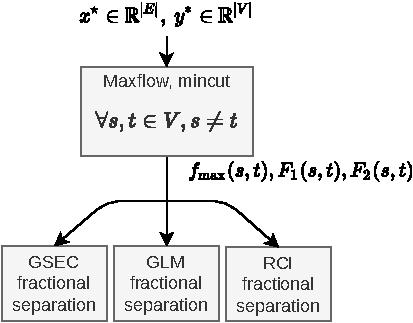
\includegraphics[width=8cm]{Imgs/fractional-separation-block-diagram.cropped.pdf}}
	\caption{A block diagram representing the structure of the employed fractional separation procedure. Recall that fractional separation occurrs only at iterations multiple of $N$. This is done to amortize the cost of the expensive maxflow/mincut procedure.}
	\label{fig:fractional-separation-block-diagram}
\end{figure}

\subsection{GSEC separation}
\label{sec:impl-gsec-separation}

\begin{quote}
	The setting of the parameters for generation of violated generalized subtour elimination constraints
	(6) can have a huge influence on the computational time for the BAC algorithm. A low threshold on
	violation will result in good lower bounds and fewer branch nodes but a slower convergence in each
	node, while the opposite is true for a high threshold. Also the number of violated cuts added in each
	iteration can influence the convergence and the time spent re-optimizing the LP-problem \cite{jepsen2008branchandcut}.
\end{quote}

Fortunately it is possible to instruct CPLEX to evaluate the cuts.
Premature branching can be performed if CPLEX deems cut ineffective independently
from user provided violation threshold.

\subsubsection{GSEC integral separation}
\label{sec:impl-gsec-integral-separation}

This is the most important separation technique, since it is mandatory to achieve feasible solutions for the CPTP problem.

By recalling the GSEC inequality as presented in Equation \eqref{eq:cptp-gsec-constraints}, and the connected components as discussed in Section \ref{sec:integral-separation}, and in Algorithm \ref{algo:cc-dfs} we can pick $S \subseteq V_0 = \left\{ i \mid cc(i) = k  \right\}   \quad \forall k \in C, k > 0$.
Note that using major connected components, i.e. subtours, the set $S$ always satisfies $\SetSize*{S} \ge 2$.
Since we are dealing with integer CPTP solutions of the form $x^*_{ij},\ y^*_{i} \in \{0, 1\}$ it is easy to see that:

\begin{align}
	\sum_{(i, j) \in \delta(S)} x^*_{ij} = 0 \\
	y_i =  1 \quad \forall i \in S
\end{align}

which imply that the GSEC inequality $\sum_{(i, j) \in \delta(S)} x_{ij} \ge 2 y_i$ cannot be satisfied by any $i \in S$.
In a single integral separation iteration we can therefore separate:
\begin{equation}
	\sum^{n_c}_{k = 1} \SetSize*{ \Set*{ i \mid cc(i) = k \quad \forall i \in V } }
\end{equation}

violated GSECs inequality, which can be promptly reported to the MIP solver to reject the candidate integral solution.

A complete pseudo-code is provided in Algorithm \ref{algo:gsec-integral-sep}.

\begin{algorithm}
	\caption{An algorithm for separating GSEC integral inequalities for the CPTP}
	\label{algo:gsec-integral-sep}
	\KwResult{$n_c$: number of subtours formed}
	\KwData{$cc[i] \in C$: connected component of $\forall i \in V$}
	\KwData{$x^*, y^* \in \{0, 1\}$: current integral solution of
		\cref{eq:cptp-static-model-0,eq:cptp-static-model-1,eq:cptp-static-model-2,eq:cptp-static-model-3,eq:cptp-static-model-4,eq:cptp-static-model-5}
	}
	\Proc{\textit{gsec\_integral\_sep}($n_c$, $cc$, $x^\star$, $y^\star$)}{
	\For{$k \gets 1$ \KwTo $n_c$}{
		\Let $S \gets  \Set* {i \mid cc[i] = k}$\;
		\Assert{$|S| \ge 2$}\;
		\Comment{Build the cut}
		\Let nnz $\gets$ 0, index $\gets$ [], value $\gets$ []\;
		\For{$e = \Set*{i, j} \in E \mid i \in S,\ j \notin S$}{
			index[nnz] $\gets$ x\_mip\_var\_idx($e$)\;
			value[nnz] $\gets$ $1$\;
			nnz $\gets$ nnz + $1$\;
		}
		\For{$i \in S$}{
			index[nnz] $\gets$ y\_mip\_var\_idx($i$)\;
			value[nnz] $\gets$ $-2.0$\;
			\Comment{Reject and report cut to MIP}
			mip\_add\_user\_cut(nnz, index, value)\;
		}
	}
}

\end{algorithm}

\subsubsection{GSEC fractional separation}
\label{sec:impl-gsec-fractional-separation}

By recalling the GSEC inequality as presented in Equation \eqref{eq:gsec-constraints}, and the discussion about separating fractional $S \subseteq V_0$ in Section \ref{sec:fractional-separation}, it is easy to see that given a fractional solution instance of the form $0 \le x^*_{ij} \le 1,\ 0 \le y^*_{i} \le 1$ we have that:

\begin{equation}
	\sum_{(i, j) \in \delta(S)} x^*_{ij} = \maxflow(s, t)
\end{equation}

where the $\maxflow(s, t)$ denotes the maximum flow computed in the fractional separation of $S \subseteq V_0$.
Therefore, if $\SetSize*{S} \ge 2$, any $i \in S$ that violates

\begin{equation}
	\maxflow(s, t) \ge 2 y_i
\end{equation}

can be used to separate a violated GSEC inequality.
Recall that the number of sets $S \subseteq V_0$ in a fractional iteration is in the order of $\Theta(N^2)$, it is possible to separate $O(N^3)$ GSECs per separation.
We noticed that, generating and reporting all the violated GSECs inequalities across al fractional separation iterations led to a slow down of the MIP solver, which was flooded with weak GSEC inequalities.

Therefore, in our implementation we took a slightly different approach, by relaxing the conditions in which GSEC inequalities are reported to the MIP.
It is important to note that relaxing the conditions in which the GSEC fractional inequalities are reported, may lead to situations in which certain indispensible inequalities fall through without ever being handled in the fractional separation procedure.
But this situation is of a little importance to us, the remaining GSEC constraints which are not caught in the fractional separation, will eventually be handled by the complete integral separation procedure.

In our implementation a GSEC inequality is separated for $S \subseteq V_0,\ \SetSize*{S} \ge 2$ only if

\begin{equation}
	\maxflow(s, t) \ge 2 y_i - \varepsilon_{\mt{GSEC}}
\end{equation}

is violated.
The $\varepsilon_{\mt{GSEC}}$ is a constant which denotes the violation tolerance for the GSEC fractional separation.
In our implementation we picked $\varepsilon_{\mt{GSEC}} = \epsGsecFValue$.
If the GSEC inequality violation does not surpass this tolerance, the GSEC inequality is not generated and reported to the MIP solver.
On top of that, to further reduce the number of generated GSECs, we report only the single most violated GSEC per set $S \subseteq V_0$ by using the customer $i \in V_0$ that maximizes the $\maxflow(s, t) - 2 y_i$ violation.

The complete pseudocode can be found in Algorithm \ref{algo:gsec-frac-sep}.

\begin{algorithm}
	\caption{An algorithm for separating GSEC fractional inequalities for the CPTP}
	\label{algo:gsec-frac-sep}
	\KwData{$\maxflow(s, t), F_1(s, t), F_2(s, t)$: maxflow and bipartitions induced from an arbitrary $s \ne t, s \in V, t \in V$ pair}
	\KwData{$x^*, y^* \in [0, 1]$: current fractional solution of \cref{eq:cptp-static-model-0,eq:cptp-static-model-1,eq:cptp-static-model-2,eq:cptp-static-model-3}}
	\Proc{\textit{gsec\_frac\_sep}($\maxflow(u, v)$, $F_1(u, v)$, $F_2(u, v)$, $x^\star$, $y^\star$)}{
	\Const sense $\gets$ '$\ge$'\;
	\Const rhs $\gets$ $0$\;
	\Const $\varepsilon_{\mt{GSEC}} \gets \epsGsecFValue$\;

	\Let $S$\;
	\uIf{$0 \notin F_1(u, v)$}{
		$S \gets F_1(u, v)$\;
	}\Else{
		$S \gets F_2(u, v)$\;
	}

	\Comment{Scan for most violated customer}
	\Let $c \gets -1$, $m \gets \infty$\;
	\For{$i \in V \mid i \in S$}{
		\Let $v \gets \maxflow(u, v) - 2 y^*_i$\;

		\If{$\Expr*{\maxflow(u, v) < 2 y^*_i - \varepsilon_{\mt{GSEC}}}$ \And $v < m$}{
			$c \gets i$\;
			$m \gets v$\;
		}
	}

	\If{$c \ge 0$ \And $|S| \ge 2$}{
		\Comment{Build the cut}
		\Let nnz $\gets$ 0, index $\gets$ [], value $\gets$ []\;
		\For{$e = \Set*{i, j} \in E \mid i \in S,\ j \notin S$}{
			index[nnz] $\gets$ x\_mip\_var\_idx($e$)\;
			value[nnz] $\gets$ $1.0$\;
			nnz $\gets$ nnz + $1$\;
		}

		index[nnz] $\gets$ y\_mip\_var\_idx($c$)\;
		value[nnz] $\gets$ $-2.0$\;
		nnz $\gets$ nnz + $1$\;
		\Comment{Reject and report cut to MIP}
		mip\_add\_user\_cut(sense, rhs, nnz, index, value)\;
	}
}

\end{algorithm}

\subsection{RCC separation}
\label{sec:impl-rcc-separation}

In this section we describe the separation of the RCC inequalities, as they were defined in Equation \eqref{eq:rcc-inequality}.
In our work we implemented both the integral and the fractional separation for this family of inequalities.
However, we will omit the detail of the integral separation in this section, since they follow naturally from ideas explained in previous sections.

The fractional separation of RCC inequalities is not any different from the separation of the GLM fractional inequalities presented in Section \ref{sec:glm-separation}.
The only difference is that the set $S \subseteq V_0$, does not need to satisfy $\SetSize*{S} \ge 2$.

Therefore, a set $\SetSize*{S} \subseteq V_0$ can separate a single RCC cut if the following inequality

\begin{equation}
	\begin{split}
		\ExprCptpFlowExiting{S} -2 \ExprCptpServedDemandWithWeight{S}{i}{\frac{q_i}{\ExprQr(S)}}    \ge   2 \left( \ceil*{ \frac{q(S)}{Q}} - \frac{q(S)}{Q_{\mathrm{R}}(S)} \right) - \varepsilon_{\mt{RCC}}
	\end{split}
\end{equation}

is violated.
The $\varepsilon_{\mt{RCC}}$ is a constant which denotes the violation tolerance for the RCC fractional separation.
In our implementation we picked $\varepsilon_{\mt{RCC}} = \epsRccFValue$.
We can separate $O(N^2)$ RCC cuts since the number of set $S \subseteq V_0$ is in the order of $\Theta(N^2)$ per fractional separation iteration.

The complete pseudocode for both the integral and fractional separation can be found in Algorithms \ref{algo:rcc-integral-sep}, \ref{algo:rcc-frac-sep} respectively.

\begin{algorithm}
	\caption{An algorithm for separating RCC integral inequalities for the CPTP}
	\label{algo:rcc-integral-sep}
	\KwResult{$n_c$: number of subtours formed}
	\KwData{$cc[i] \in C$: connected component of $\forall i \in V$}
	\KwData{$x^*, y^* \in \{0, 1\}$: current integral solution of
		\cref{eq:cptp-static-model-0,eq:cptp-static-model-1,eq:cptp-static-model-2,eq:cptp-static-model-3,eq:cptp-static-model-4,eq:cptp-static-model-5}
	}
	\Proc{\textit{rcc\_integral\_sep}($n_c$, $cc$, $x^\star$, $y^\star$)}{
	\Const sense $\gets$ '$\ge$'\;

	\For{$k \gets 1$ \KwTo $n_c$}{
		\Const $S \gets  \Set* {i \mid cc[i] = k}$\;
		\Const $Q_S$ $\gets \sum\limits_{i \in S} q_i$\;
		\Const $Q_R$ $\gets$ $\mod(Q_S, Q)$\;
		\Const rhs $\gets$ $2 \Expr*{\ceil*{\frac{Q_S}{Q}} - \frac{Q_S}{Q_R}}$\;

		\If{$Q_R > 0$ \And $|S| \ge 1$}{
			\If{$-2 \sum\limits_{i \in S} \frac{q_i}{Q_R} y^*_i  < $ rhs}{
				\Comment{Build the cut}
				\Let nnz $\gets$ 0, index $\gets$ [], value $\gets$ []\;
				\For{$e = \Set*{i, j} \in E \mid i \in S,\ j \notin S$}{
					index[nnz] $\gets$ x\_mip\_var\_idx($e$)\;
					value[nnz] $\gets$ $1$\;
					nnz $\gets$ nnz + $1$\;
				}
				\For{$i \in S$}{
					index[nnz] $\gets$ y\_mip\_var\_idx($i$)\;
					value[nnz] $\gets$ $-2 q_i / Q_R$\;
					nnz $\gets$ nnz + $1$\;
				}
				\Comment{Reject and report cut to MIP}
				mip\_add\_user\_cut(sense, rhs, nnz, index, value)\;
			}
		}
	}
}

\end{algorithm}

\begin{algorithm}
	\caption{An algorithm for separating RCC fractional inequalities for the CPTP}
	\label{algo:rcc-frac-sep}
	\KwData{$\maxflow(s, t), F_1(s, t), F_2(s, t)$: maxflow and bipartitions induced from an arbitrary $s \ne t, s \in V, t \in V$ pair}
	\KwData{$x^*, y^* \in [0, 1]$: current fractional solution of
		\cref{eq:cptp-static-model-0,eq:cptp-static-model-1,eq:cptp-static-model-2,eq:cptp-static-model-3}
	}
	\Proc{\textit{rcc\_frac\_sep}($n_c$, $cc$, $x^*$, $y^*$)}{
	\Const $\varepsilon_{\mt{RCI}} \gets \epsRccFValue$\;

	\For{$c \gets 1$ \KwTo $n_c$}{
		\Let $S$\;
		\uIf{$0 \notin F_1(s, t)$}{
			$S \gets F_1(s, t)$\;
		}\Else{
			$S \gets F_2(s, t)$\;
		}
		\Let $Q_S$ $\gets \sum_{i \in S} q_i$\;
		\Let $S_S$ $\gets \sum_{i \in S} y^*_i \cdot q_i$\;
		\Let $Q_R$ $\gets$ $\mod(Q_S, Q)$\;
		\If{$Q_R > 0$ \And $|S| \ge 1$}{
			\If{$\maxflow(s, t) -2 S_S / Q_R$ $<$ $2 \ceil*{Q_S / Q} - 2 Q_S / Q_R$ - $\varepsilon_{\mt{RCI}}$}{
				\Comment{Build the cut}
				\Let nnz $\gets$ 0, index $\gets$ [], value $\gets$ []\;
				\For{$i \in V \mid i \in S$}{
					index[nnz] $\gets$ y\_mip\_var\_idx($i$)\;
					value[nnz] $\gets$ $-2 q_i / Q_R$\;
					nnz $\gets$ nnz + $1$\;

					\For{$j \in V \mid j \notin S$}{
						index[nnz] $\gets$ x\_mip\_var\_idx($i$, $j$)\;
						value[nnz] $\gets$ $1$\;
						nnz $\gets$ nnz + $1$\;
					}
				}
				\Comment{Reject and report cut to MIP}
				mip\_add\_user\_cut(nnz, index, value)\;
			}
		}
	}
}

\end{algorithm}

\subsection{GLM separation}
\label{sec:impl-glm-separation}

In this section we describe the separation of the GLM inequalities, as they were defined in Equation \eqref{eq:glm-inequality}.
In our work we implemented both the integral and the fractional separation for this family of inequalities.
However, in this section we will explain only the fractional separation and we will omit the details about integral separation.
The integral separation follows naturally from adapting the ideas that will here after be presented in this section, and by employing a similar reasoning as was done in Section \ref{sec:gsec-integral-separation}, for the GSEC inequalities (i.e. using the connected components).

Let $F_1(s, t),\ F_2(s, t)$ be the bipartition induced in solving the min-cut problem as was presented in Section \ref{sec:fractional-separation}.
Again we showed that we can pick a valid $S \subseteq V_0$ in the following way

\begin{equation}
	S \subseteq V_0 =
	\begin{cases}
		F_1(s, t), & \texttt{if } 0 \notin F_1 \\
		F_2(s, t), & \texttt{otherwise}
	\end{cases}
\end{equation}

In case of the integral separation the same reasoning apply here, but instead of using the min-cut bipartition, we use the connected components array to find a valid $S \subseteq V_0$.

We need to count the number of vertices $i$ in $S$ to verify that indeed $\SetSize*{S} \ge 2$.
If $\SetSize*{S} < 2$, no GLM inequalities can be separated.
Otherwise a single GLM cut can be separated if the following inequality

\begin{equation}
	\begin{split}
		\ExprCptpFlowExitingWithWeight{S}{\Expr*{1 - 2 \frac{q_j}{Q}}} - 2 	\ExprCptpServedDemandWithWeight{S}{i}{\frac{q_i}{Q}} \ge - \varepsilon_{\mt{GLM}}
	\end{split}
\end{equation}

is violated.
The $\varepsilon_{\mt{GLM}}$ is a constant which denotes the violation tolerance for the GLM fractional separation.
In our implementation we picked $\varepsilon_{\mt{GLM}} = \epsGlmFValue$.
We can separate $O(N^2)$ GLM cuts since the number of set $S \subseteq V_0$ is in the order of $\Theta(N^2)$ per fractional separation iteration.

The complete pseudocode for both the integral and fractional separation can be found in Algorithms \ref{algo:glm-integral-sep}, \ref{algo:glm-frac-sep} respectively.

\begin{algorithm}
	\caption{An algorithm for separating GLM integral inequalities for the CPTP}
	\label{algo:glm-integral-sep}
	\KwResult{$n_c$: number of subtours formed}
	\KwData{$cc[i] \in C$: connected component of $\forall i \in V$}
	\KwData{$x^*, y^* \in \{0, 1\}$: current integral solution of
		\cref{eq:cptp-static-model-0,eq:cptp-static-model-1,eq:cptp-static-model-2,eq:cptp-static-model-3,eq:cptp-static-model-4,eq:cptp-static-model-5}
	}
	\Proc{\textit{glm\_integral\_sep}($n_c$, $cc$, $x^*$, $y^*$)}{
	\Const $\varepsilon_{\mt{GLM}} \gets 0.01$\;

	\For{$c \gets 1$ \KwTo $n_c$}{
		\Let $S \gets  \Set* {i \mid cc[i] = c}$\;
		\If{$|S| \ge 2$}{
			\Comment{Build the cut}
			\Let lhs $\gets 0$\;
			\Let nnz $\gets$ 0, index $\gets$ [], value $\gets$ []\;
			\For{$i \in V \mid i \in S$}{
				\For{$j \in V \mid j \notin S$}{
					index[nnz] $\gets$ x\_mip\_var\_idx($i$, $j$)\;
					value[nnz] $\gets$ $1 - 2 q_j / Q$\;
					lhs $\gets$ lhs + $x^*_{ij} \cdot (1 - 2 q_j / Q)$\;
					nnz $\gets$ nnz + $1$\;
				}
			}
			\For{$i \in V \mid i \in S$}{
				index[nnz] $\gets$ y\_mip\_var\_idx($i$)\;
				value[nnz] $\gets$ $-2 q_i / Q$\;
				lhs $\gets$ lhs + $y^*_{i} \cdot (2 q_i / Q)$\;
				nnz $\gets$ nnz + $1$\;
			}
			\If{\Not lhs $\ge$ $-\varepsilon_{\mt{GLM}}$}{
				\Comment{Reject and report cut to MIP}
				mip\_add\_user\_cut(nnz, index, value)\;
			}
		}
	}
}

\end{algorithm}

\begin{algorithm}
	\caption{An algorithm for separating GLM fractional inequalities for the CPTP}
	\label{algo:glm-frac-sep}
	\KwData{$\maxflow(s, t), F_1(s, t), F_2(s, t)$: maxflow and bipartitions induced from an arbitrary $s \ne t, s \in V, t \in V$ pair}
	\KwData{$x^*, y^* \in [0, 1]$: current fractional solution of
		\cref{eq:cptp-static-model-0,eq:cptp-static-model-1,eq:cptp-static-model-2,eq:cptp-static-model-3}
	}
	\Proc{\textit{glm\_frac\_sep}($\maxflow(u, v)$, $F_1(u, v)$, $F_2(u, v)$, $x^\star$, $y^\star$)}{
	\Const sense $\gets$ '$\ge$'\;
	\Const rhs $\gets$ $0$\;
	\Const $\varepsilon_{\mt{GLM}} \gets \epsGlmFValue$\;
	\Let $S$\;
	\uIf{$0 \notin F_1(u, v)$}{
		$S \gets F_1(u, v)$\;
	}\Else{
		$S \gets F_2(u, v)$\;
	}

	\If{$|S| \ge 2$}{
		\Comment{Build the cut}
		\Let lhs $\gets 0$\;
		\Let nnz $\gets$ 0, index $\gets$ [], value $\gets$ []\;
		\For{$i \in V \mid i \in S$}{
			\For{$j \in V \mid j \notin S$}{
				index[nnz] $\gets$ x\_mip\_var\_idx($i$, $j$)\;
				value[nnz] $\gets$ $1 - 2 q_j / Q$\;
				lhs $\gets$ lhs + $x^\star_{ij} \cdot (1 - 2 q_j / Q)$\;
				nnz $\gets$ nnz + $1$\;
			}
		}
		\For{$i \in V \mid i \in S$}{
			index[nnz] $\gets$ y\_mip\_var\_idx($i$)\;
			value[nnz] $\gets$ $-2 q_i / Q$\;
			lhs $\gets$ lhs + $y^*_{i} \cdot (2 q_i / Q)$\;
			nnz $\gets$ nnz + $1$\;
		}
		\If{\Not lhs $\ge$ $-\varepsilon_{\mt{GLM}}$}{
			\Comment{Reject and report cut to MIP}
			mip\_add\_user\_cut(sense, rhs, nnz, index, value)\;
		}
	}
}

\end{algorithm}
